\section{Monitoring}

\begin{figure}
\centering
\fbox{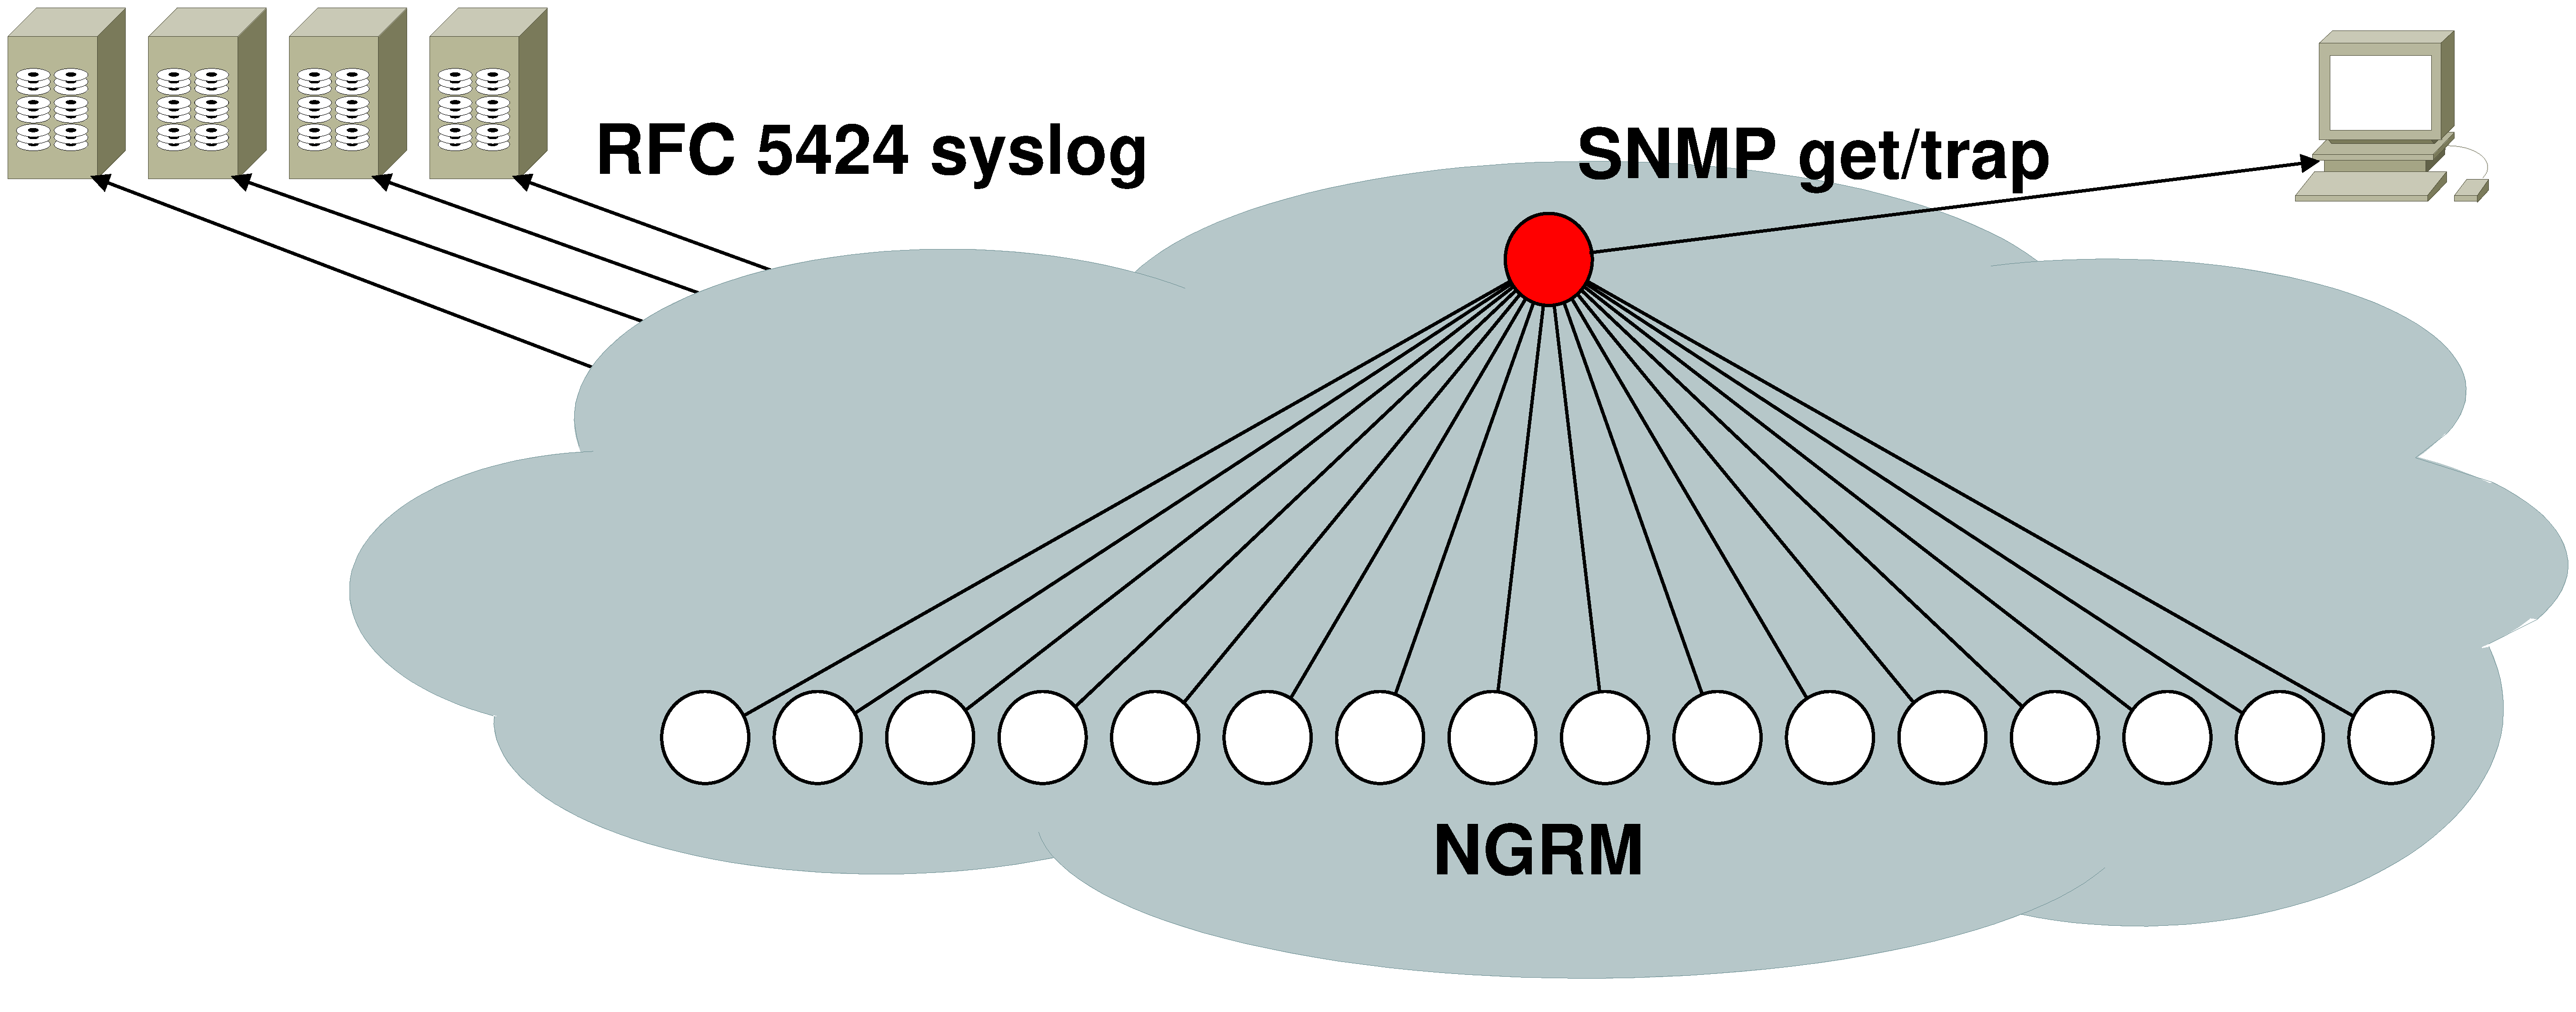
\includegraphics[scale=0.1]{../fig/mon_iface.eps}}
\caption{The \ngrm\ monitoring system interfaces with an external
enterprise monitoring system using SNMP, and with a persistent log
database using RFC 5424 structured syslog.}
\label{FigMonExt}
\end{figure}

The primary function of \ngrm's integrated monitoring is resource
health tracking.  This information is required in real time by schedulers
and runtimes to ensure that work is not launched on broken resources,
and that when things do go wrong, appropriate action can be taken.
In addition, \ngrm\ monitoring can be extended and customized
by sys admins and job owners to cover additional monitoring needs
that may be site, hardware, or job specific
(\ref{ReqsHiLevFun} req. 3.1).
Ideally \ngrm\ will be flexible enough to meet all
monitoring data aquisition requirements on compute nodes,
where our model is to synchronize monitoring interruptions within each job
and allow the system noise impact of monitoring to be tuned by the job owner
(\ref{ReqsHiLevFun} req. 3.0 and 3.2).

As shown in Figure~\ref{FigMonExt}, monitoring interfaces with an external
log database and enterprise monitoring system.
The log database is intended to be a comprehensive, schemaless, site-wide
store that will support a high insertion rate, large storage capacity,
and scalable queries.
As a record of all events in the data center, it will facilitate
post-mortem analysis, enabling the correlation of job data
with occurrences that were not actively tracked by the job during its
execution, thus not part of the canonical job record.
Users will be permitted to inject application-level information into this
store and perform analysis as well
(\ref{ReqsHiLevFun} req. 3.6).

The enterprise monitoring system is the mechanism used by operations center
staff and system administrators to monitor site systems which might include
\ngrm\ as well as facilities, network devices, storage appliances,
and non-\ngrm\ clusters.
This system is likely to already be in place at a site, thus common
protocols are chosen to reduce the effort required to integrate with \ngrm.

Monitoring state for a job is stored in the {\em resource database}, and
fault events are recorded in the {\em job database}.
These databases provide extensibility and persistency features described
in Section~\ref{sect:resdb} and \ref{sect:jobdb}.
Monitoring follows the \ngrm\ job recursion pattern, and is layered upon
the comms framework.  Recall from the Section~\ref{sect:commsIP} that
each comms session/job has a unique domain name within the \ngrm\ private
DNS namespace.  Live monitoring data can be obtained by using the resource
manager API to query the resource and job databases on the job's control
node, using its domain name.

Within a job, some applications and runtimes will require notification
when system faults occur.
For example, when a node that is part of a job crashes, some applications
may be able to request a replacement node and continue.
To facilitate fault notification within a job, \ngrm\ will
implement the CIFTS Fault Tolerance Backplane API\cite{FTBAPI} (FTB-API),
an emerging standard for fault notification available in some MPI
implementations and other software.
Using FTB-API, applications and runtimes can produce and consume fault
events within the job using its publish/subscribe interface, which we layer on
top of our comms event messaging service.  Furthermore, a gateway is provided
on the job control node which allows software within the job to subscribe
to faults generated externally (such as by a file system used by the job),
and to publish certain faults that may be of interest to others.

\ngrm\ Monitoring thus consists of
the plugin framework, 
log database interface,
enterprise monitoring interface,
and FTB-API interface.
Each of these parts is discussed below.

\subsection{Plugin Framework}

\begin{figure}
\begin{minipage}[b]{0.4\linewidth}
\fbox{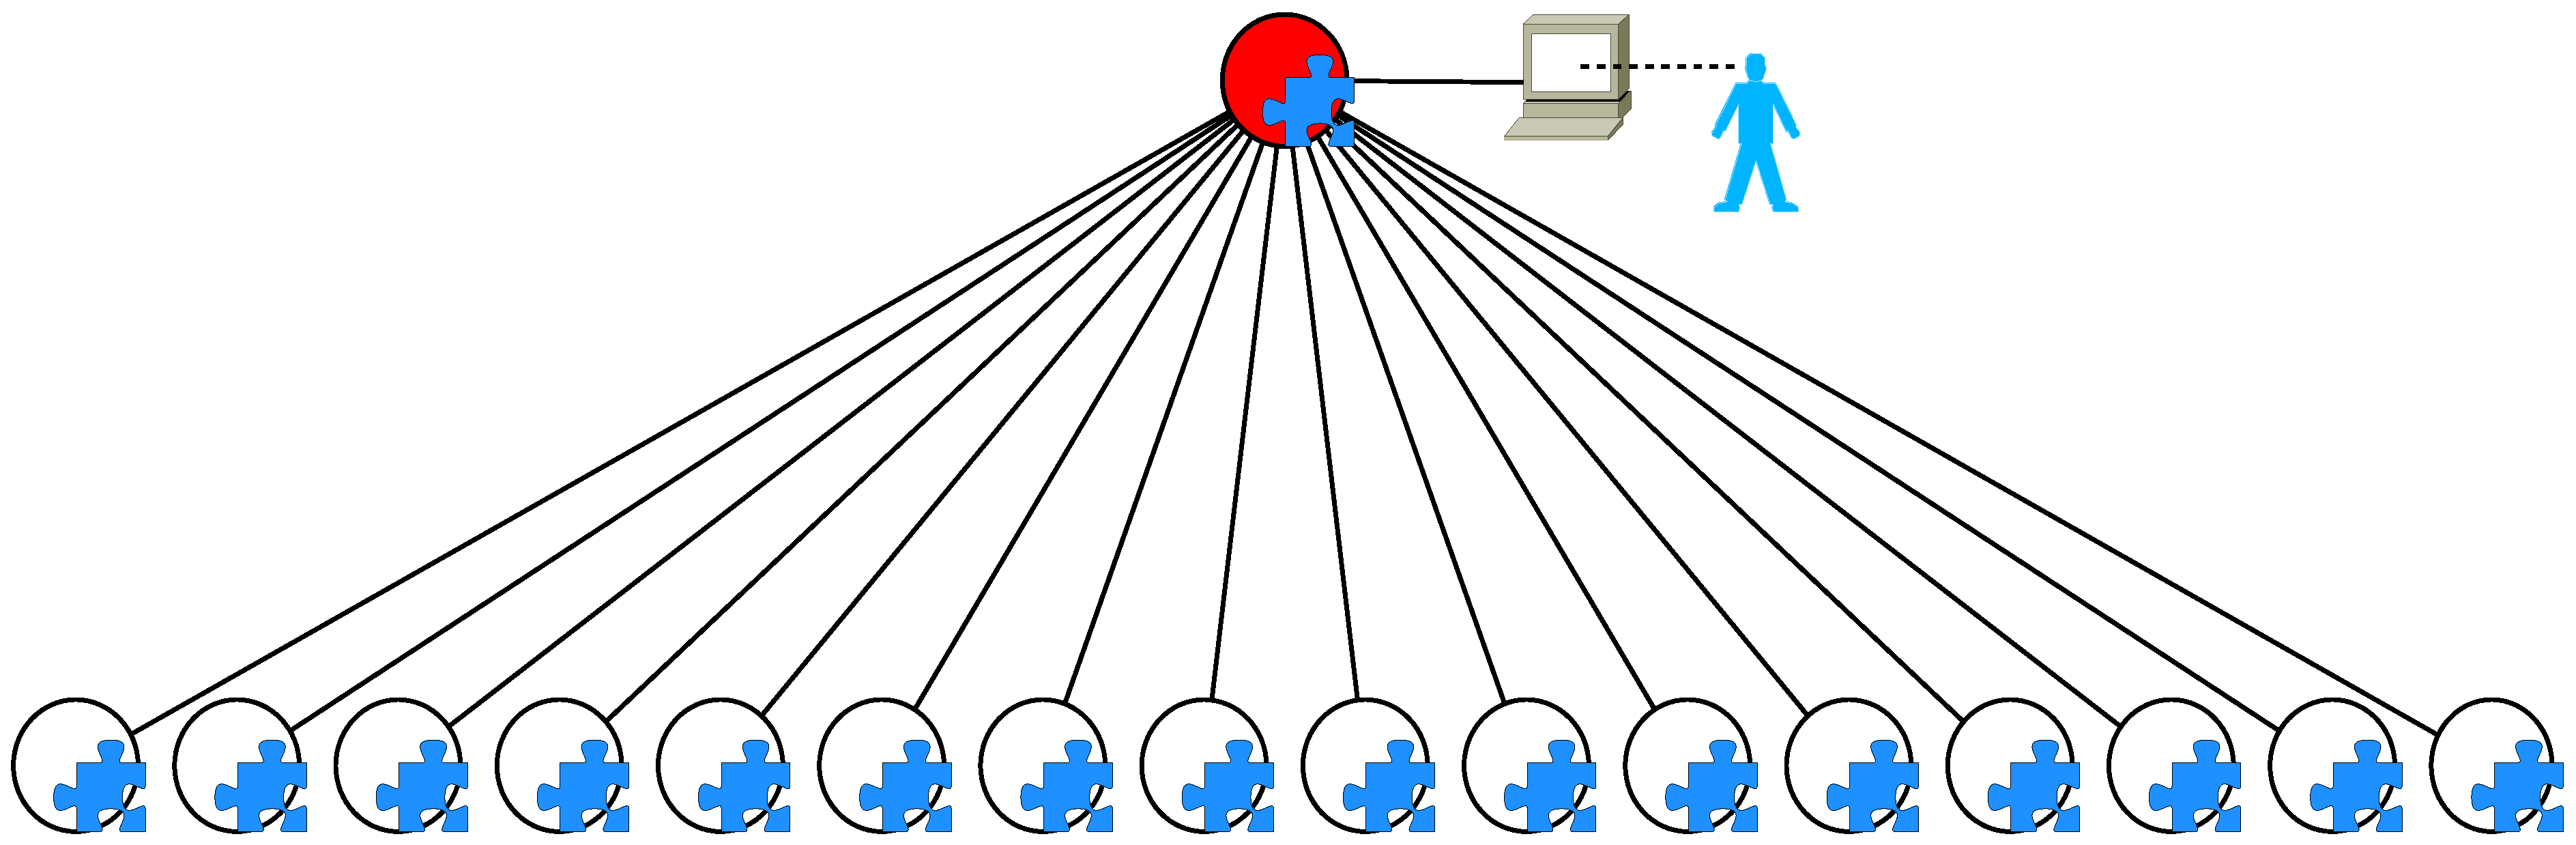
\includegraphics[scale=0.1]{../fig/mon_ex1a.eps}}
\end{minipage}
\hspace{1cm}
\begin{minipage}[b]{0.4\linewidth}
\fbox{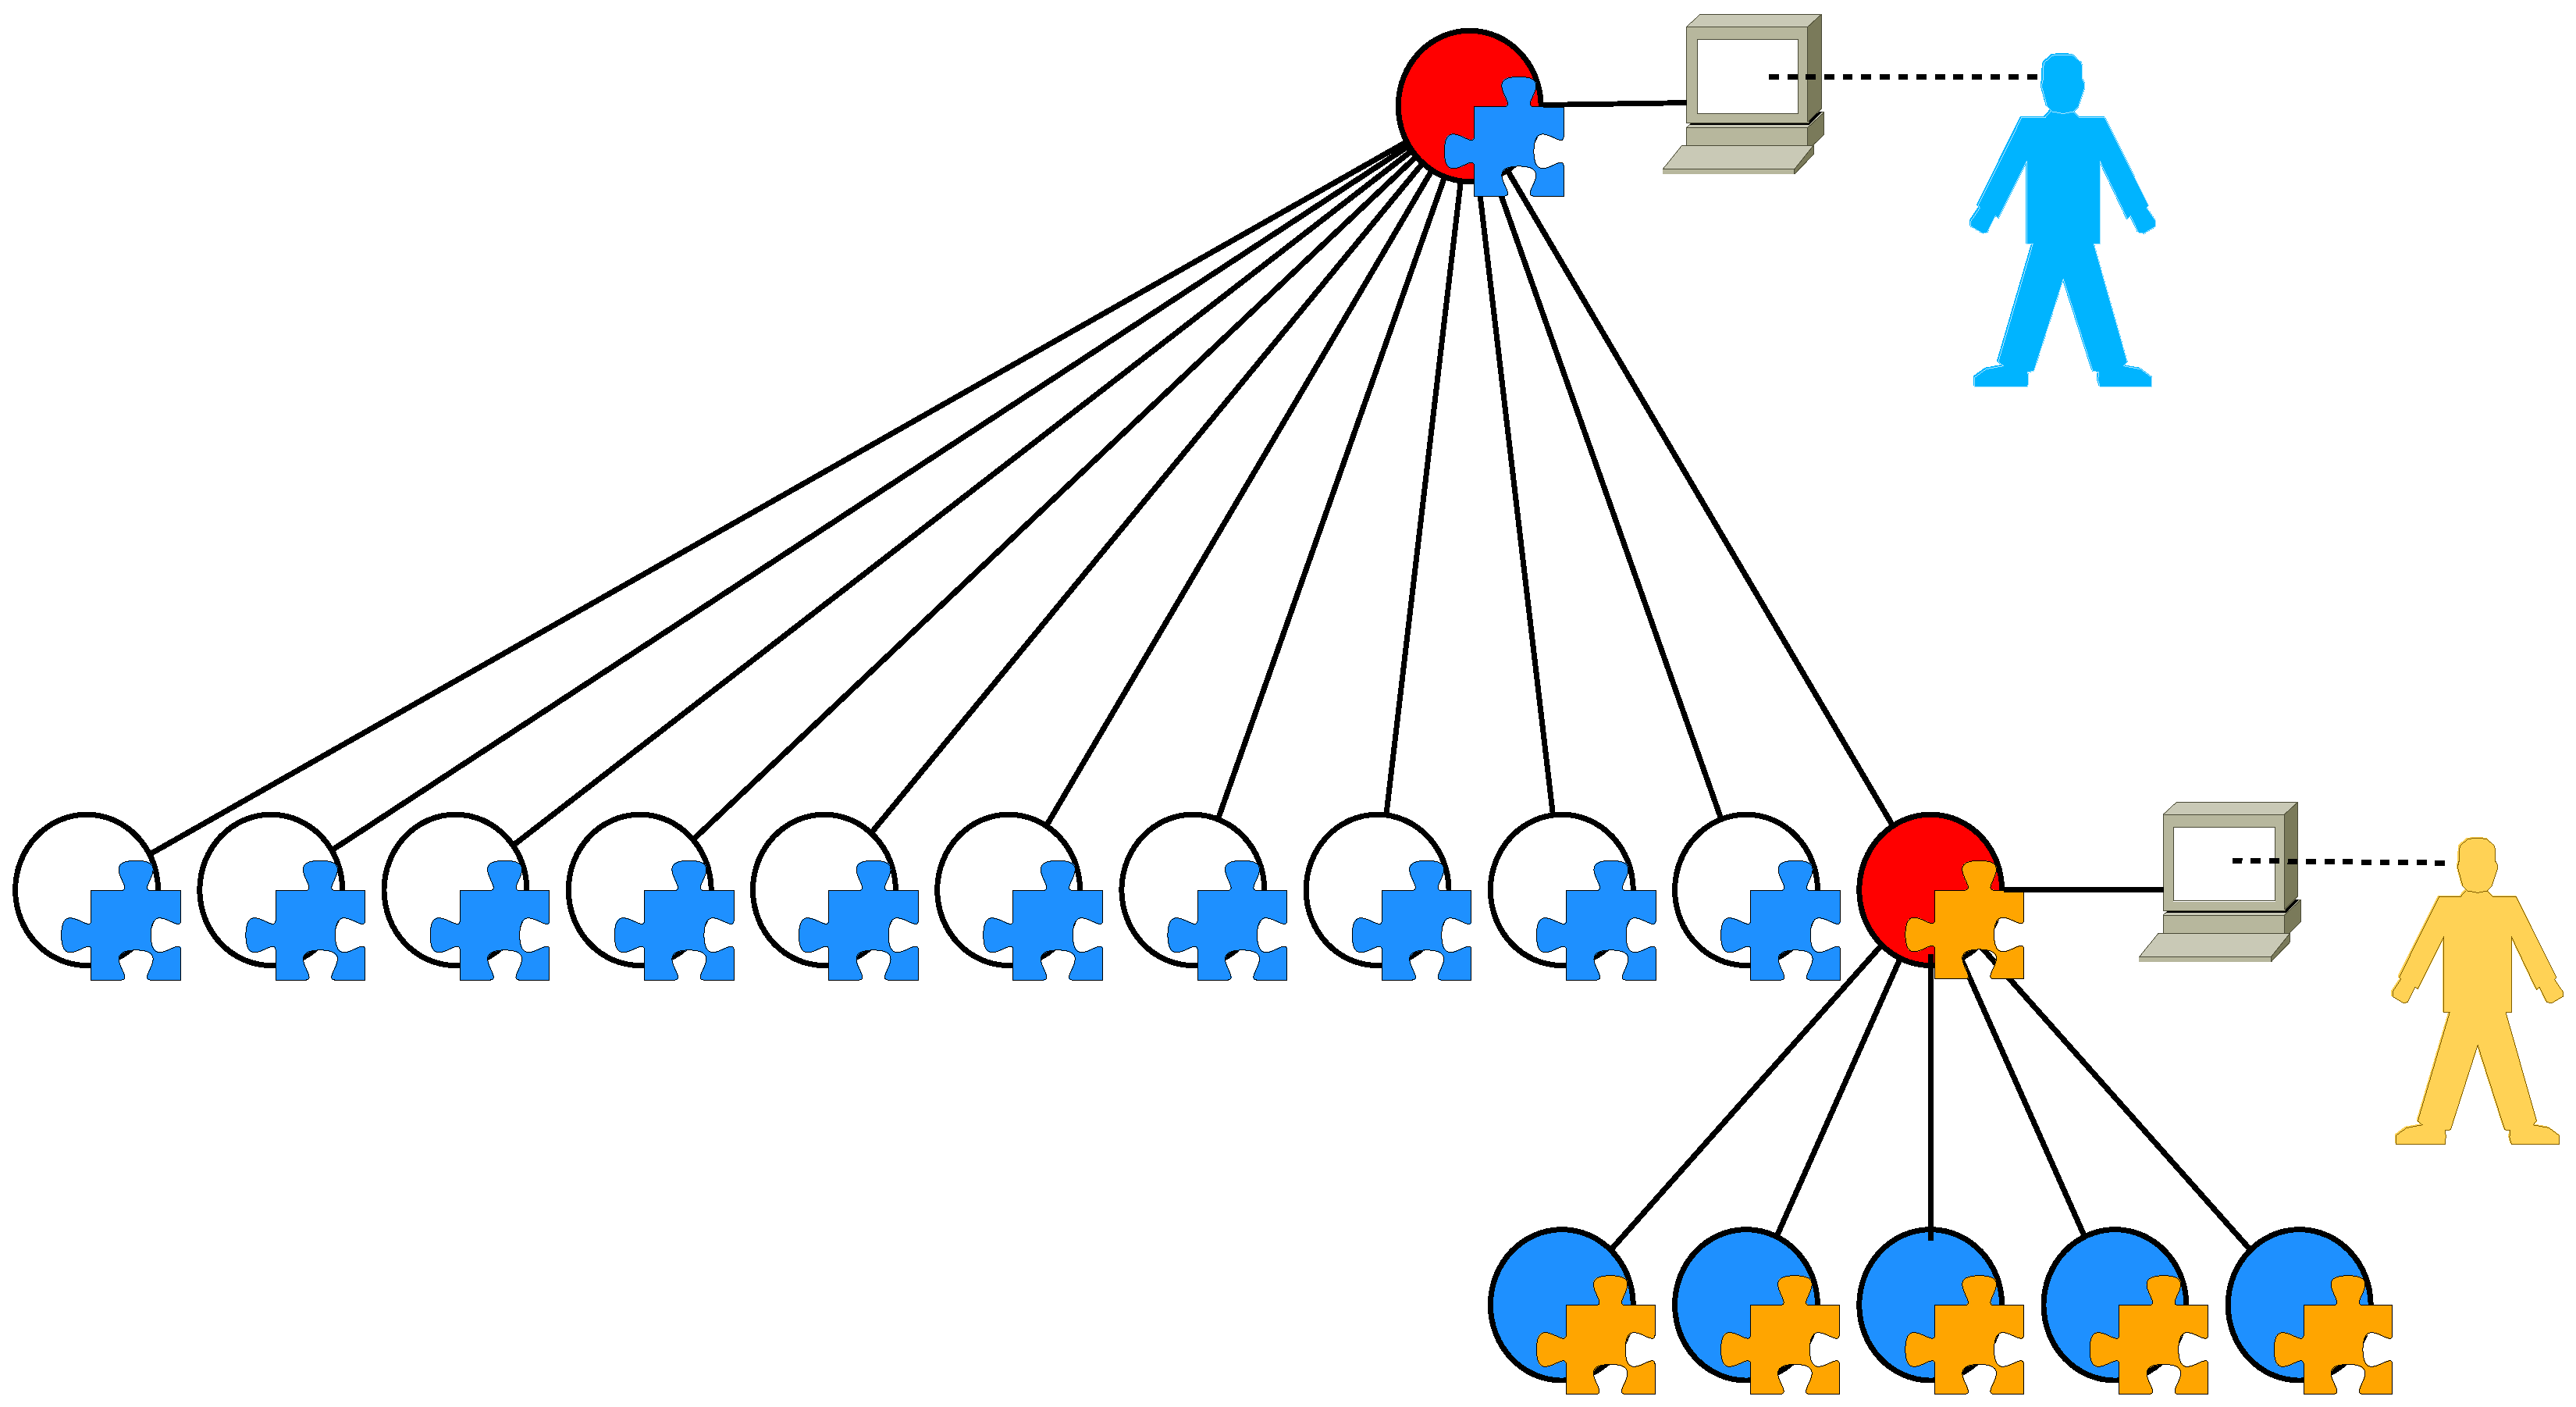
\includegraphics[scale=0.1]{../fig/mon_ex1b.eps}}
\end{minipage}
\caption{Monitoring follows the session/job hierarchy.
Control nodes (red) export a web-based monitoring interface for each job.
The monitoring plugin stack (jigsaw pieces) is customizable for each job.
Plugin execution is coordinated by the job's scheduling trigger event.}
\label{FigMonEx1}
\end{figure}

The monitoring plugin system provides a facility for arbitrary code to be
periodically executed across a session.  To minimize disruption to
bulk-synchronous workloads, this execution is synchronized by the 
session scheduling trigger event.  The set of active plugins is
under the control of the session owner, with some reasonable
defaults provided that can be overridden.  The plugin framework is
depicted in Figure~\ref{FigMonEx1}.

%The details of the plugin structure is a design activity, however,
%an example of a possible solution is for plugins to take the form of
%Lua scripts loaded into the CMB state database
%(thus shared across the session) and executed in the context of
%a monitoring daemon with an embedded Lua interpreter.

Plugins have three main functions: data source, data reduction,
and data sink.  The data source function is driven by the scheduling
trigger and may directly publish events, for example if a monitored
value exceeds a threshold, or produce structured data for the
aggregation/reduction network.
The data reduction function aggregates structured data from instances
of the plugin's source function.
For example, a plugin that monitors the total amount of memory used
by the session might register a reduction function that takes the sum of
arriving samples.
Finally, plugins can register a function to sink data at the monitoring
console, rendering it for display, or at points in the session that interface
with the monitoring database for persistent storage.

\subsection{Log Database Interface}

The monitoring database will be a large, centralized, persistent database
that stores structured log data for analysis and data provenance.
Log data is generated by monitoring plugins, but may come from other sources
such as syslog, the \ngrm\ runtime, resource manager, or scheduler.

One reason this database is centralized is to allow queries
to be constructed that correlate failures or performance anomalies
across domains; for example, jobs running slow or producing incorrect
results because of file system problems.  The database will directly
benefit system administrators and suport staff who currently perform
these tasks manually.

By preserving contextual information surrounding the execution of a job,
we enable questions to be asked later on when the same job produces
different results.  This is a central goal of provenance.

The database will need some schema design in order to enable queries
that are operationally useful.  For example, RAS metrics may be obtained
on hardware component failures if we are careful to log enough information
to identify the component (e.g. a double bit memory error at address \#xxxx
versus a failure of dimm with model and serial number).

This effort will leverage the work of an in-progress LDRD
feasbility study\cite{LogLDRD}.

\subsection{Enterprise Monitoring Interface}

\subsection{FTB-API Interface}

\subsection{Monitoring WBS}

\begin{longtable}{|p{1cm}|p{10.2cm}|p{1cm}|p{1cm}|p{1.8cm}|}\hline
  \textbf{Item} & \textbf{Description}
                & \textbf{Deliv}\footnote{SD = software drop,
                        DR = design review, V = viewgraphs, D = document}
                & \textbf{Weeks} & \textbf{Depend} \\
  \hline
  \hline
  \multicolumn{5}{|l|}{3.3. \textbf{Monitoring Plugin System}} \\
  \hline
  3.3.1.& Design/prototype plugin system including structured log format
	  and event naming.  (See also possible CIFTS/FTB tie-in in runtime).
          (See also Meyer monitoring project).
	& DR
	&
	& comms \\
  \hline
  3.3.2.& Implement plugin system.
        & SD
        &
        & 3.3.1 \\
  \hline
  3.3.3.& Document process for creating monitoring plugins.
        & D
        &
        & 3.3.1 \\
  \hline
  3.3.4.& Design/prototype a set of default plugins including plugins
          for instrumenting jobs to gather "implicit provenance" such as
          file accesses.
        & DR
        & 
        & 3.3.1 \\
  \hline
  3.3.5 & Implement set of default plugins.
        & SD
        &
        & 3.3.4 \\

  \hline
  \multicolumn{5}{|l|}{3.4. \textbf{Monitoring Console}} \\
  \hline

  3.4.1.& Design/prototype HTTP/REST monitoring console.
          (Long/Martinez Lorenz team)
          (See also Meyer monitoring project).
	& DR
	&
	& 3.3.1 \\
  \hline
  3.4.2.& Implement monitoring console.
	& SD
	&
	& 3.3.1, 3.4.1 \\
  \hline
  3.4.3.& Design/prototype Lorenz integration.
	  Think about how monitoring console integrates with the myllnl
	  dashboard experience.
          (Long/Martinez Lorenz team)
	& DR
	&
	& 3.4.1 \\
  \hline
  3.4.4.& Design/prototype skummee integration.
          How will \ngrm\ integrate with ops monitoring view?
          How will out of band monitoring (IPMI, DDN's, etc) integrate with
	  monitoring console?
          (Meyer monitoring project).
	& DR
	&
	& 3.4.1 \\
  \hline
  3.4.5.& Implement Lorenz/skummee integration.
	& SD
	&
	& 3.4.3, 3.4.4 \\
  \hline
  \multicolumn{5}{|l|}{3.5. \textbf{Monitoring Database Interface}} \\
  \hline
  3.5.1.& Study available NoSQL databases for 100K node scalability
          and appropriate query interface.
          Use offline log data to investigate system diagnostic capability
          and prototype queries.
          (Gamblin/Mohror HPC Data Analytics FY12 LDRD)
        & V
        & 
        & LDRD \\
  \hline
  3.5.2.& Implement prototype database tied to live log sources.
          Study scalability and develop queries.
          (Gamblin/Mohror HPC Data Analytics FY12 LDRD)
          (See also: Faaland SPLUNK deployment).
        & DR
        & 
        & 3.5.1 \\
  \hline
  3.5.3.& Design/prototype access-role based security.
        & DR
        & 
        & 3.5.2 \\
  \hline
  3.5.4.& Design/prototype schemas and queries for reporting
          RAS metrics of interest to center management.
        & DR
        & 
        & 3.5.2 \\
  \hline
  3.5.5.& Design/prototype procedure for sanitizing and releasing data
	  for research study and citation.
        & DR
        & 
        & 3.5.2 \\
  \hline
  3.5.6.& Design/prototype schema for job logs and queries for
          associating job data, system log data, etc..
        & DR
        & 
        & RM, 3.5.2 \\
  \hline
  3.5.7.& Implement database.
        & SD
        & 
        & 3.5.2, 3.5.3, 3.5.4, 3.5.5, 3.5.6 \\
  \hline
\end{longtable}


